\documentclass[a4paper]{article}
\usepackage{graphicx}
\usepackage{hyperref}
\usepackage{authblk}
\usepackage{multirow}

\title{Semi-automatic staging area for high-quality structured data extraction from scientific literature}
\author[1,2]{Luca Foppiano}
\author[1]{Tomoya Mato}
\author[3]{Kensei Terashima}
\author[4]{Pedro Ortiz Suarez}
\author[3]{Tou Taku}
\author[3]{Chikako Sakai}
\author[3]{Wei-Sheng Wang}
\author[2]{Toshiyuki Amagasa}
\author[3]{Takano Yoshihiko}
\author[1]{Ishii Masashi}
\affil[1]{Materials Modelling Group, Data-driven Materials Research Field, Centre for Basic Research on Materials, NIMS, Japan}
\affil[2]{Knowledge and Data Engineering, Centre for Computational Sciences, University of Tsukuba, Japan}
\affil[3]{Frontier Superconducting Materials Group, MANA, NIMS, Tsukuba, Japan}
\affil[4]{DFKI GmbH, Germany}

\begin{document}

\maketitle

\begin{abstract}
    TBA
\end{abstract}

\section{Introduction}

The emergence of new methodologies using machine learning for materials exploration has given rise to a growing research area called materials informatics (MI) ~\cite{10.3389/fchem.2022.930369}.
This field leverages the knowledge of the materials data accumulated in the past to efficiently screen candidates of the materials with desired properties.
As a matter of course, such an approach requires a larger number of material-related data for training models.
Researchers have been developing large aggregated databases of physical properties generated by first-principles calculations based on density functional theory (DFT), such as Materials Project~\cite{materialsprojectJain2013}, JARVIS~\cite{aflowcurtarolo2012aflow}, NOMAD~\cite{nomad}, and so on, that played a role of a solid driving force for the development of materials informatics.
However, such DFT-based physical property values are not necessarily always valid, since they are derived by a certain approximation of many-body interactions in solids.
Therefore, the applicability of such calculated data is still challenging for building a machine-learned model of complicated physical properties like superconductivity.
Despite the rapid growth in scientific publications, including the exponential rise in materials science~\cite{Pratheepan_2019}, there is a scarcity of accumulated datasets of experimental data. 
The limited resources available, such as the Pauling File~\cite{Blokhin2018ThePF_paulingFile} and SuperCon~\cite{SuperCon}, have resulted in the reliance on manual extraction methods.
This could be attributed to the lack of adequate infrastructure and expertise in the field.

% The lack of adequate infrastructure and expertise could have led to creation of a single manual procedure that can extract information from diverse sources like plots, tables, and text all at once. However, while this approach may be viable in the short term, its sustainability diminishes over time. 
% On the other hand, constructing an automated process to accomplish this task presents many challenges. In the case of scientific publications, plots, tables, and text necessitates different treatments, and the resulting outputs must be merged and verified manually. Despite the challenges, it is possible to transition gradually towards automation by implementing iterative steps. This iterative approach involves reducing human involvement progressively while simultaneously optimising the efficiency of required human actions. 

SuperCon~\cite{SuperCon} was built manually over more than a decade by the National Institute for Materials Science (NIMS) in Japan and it is considered the gold standard in superconductors research.
Despite being praised for its excellent quality in numerous reports~\cite{roter2020predicting, stanev_machine_2017, tran2022machine, konno2021deep}, the updates of SuperCon have become increasingly challenging due to the high publication rate. However, in response to the need for a more efficient approach to sustain productivity, we embarked on the development of an automated system for extracting material and property information from the text contained in relevant scientific publications~\cite{lfoppiano2023automatic}. This automated process enabled the rapid creation of SuperCon\textsuperscript{2}, a comprehensive database of superconductors containing over 35,000 entries, within an operational duration of just a few days. 

Ensuring the same quality as SuperCon while automating the extraction of structured superconductors data poses significant challenges. 
We developed a web interface designed to facilitate the curation process, involving the active and ongoing management of data through its lifecycle of interest, specifically tailored for our superconductors database but open to the potential adaptation of other data structures. 
Our interface aims to maintain quality, add value, and provide for reuse over time while making the curation process more effective, and user-friendly.

There are several tools for data annotation, such as Inception~\cite{klie-etal-2018-inception}, and Doccano~\cite{doccano}, at the moment of writing this article, we are not aware of any other curation tools for materials extracted databases. 
This paper introduces our curation tool, SuperCon\textsuperscript{2}, which serves as a data staging area for SuperCon. 
The tool allows for the visualisation, correction, and integration of automatically extracted data into the SuperCon database while triggering a feedback loop to improve the machine learning (ML) models.

Our contributions to the field can be summarised as follows:
\begin{itemize}
    \item A new interface to curate and validate automatically extracted materials databases. We measured and reported an improved accuracy as compared with the manual method.
    \item a scalable ingestion process for creating a persistent database of superconductors materials and their related properties.
    \item an integrated simple anomaly detection process for the identification of outliers in the materials-properties database, 
    \item an enhanced PDF document viewer~\cite{wang2022hammer} applied to materials science, showing the materials entities from the extracted database. 
    \item the mechanism that generates training data based on curation which selects more relevant data for improving the ML models.
\end{itemize}

The subsequent section (Section~\ref{sec:ingestion}) discuss the ingestion process and the data model, then in Section~\ref{sec:user-interface} we illustrate the interface, Section~\ref{sec:data-correction} describes the data correction for automatically extracted entities, anomaly detection and the interface evaluation. 


\section{Ingestion process}
\label{sec:ingestion}

The ingestion process (Figure~\ref{fig:map-reduce}) is designed using a Map-Reduce approach. 
We briefly introduced it in our previous work~\cite{lfoppiano2023automatic} and we discuss the technical details in this section. 

\begin{figure}[ht]
  \centering
  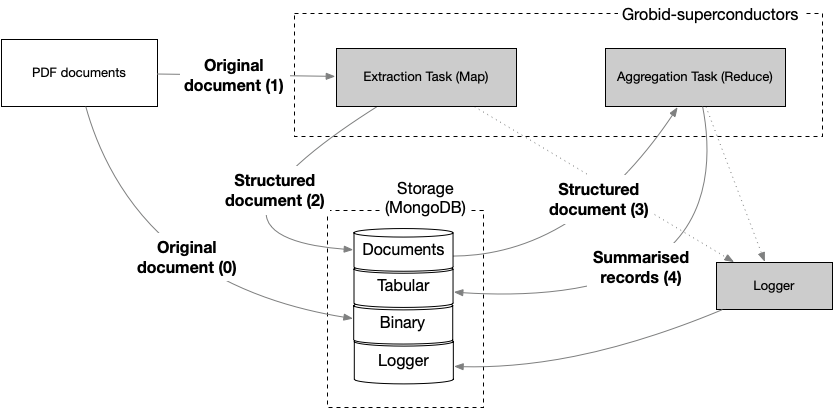
\includegraphics[width=\textwidth]{images/ingestion-schema.png} 
  \caption{Ingestion process}
  \label{fig:map-reduce}
\end{figure}


The "Extraction Task" (Map) takes the PDF documents as input, saves them, and then processes them with Grobid-superconductors. 
Grobid-superconductors transforms the PDF documents into a rich representation document including annotations and layout tokens as JSON files, which we will refer to as \textit{structured documents}.  
The "Aggregation Task" (Reduce) takes in input the structured document and reduces it to a table format where each row (we refer to as a \textit{summarised record}, or, simply \textit{record}) contains one material-tc-properties triplet.

\subsection{Architecture}
\label{sec:architecture}

The two tasks are implemented by two Python scripts that can run asynchronously and with configurable scalability.
The storage is implemented using MongoDB~\footnote{\url{https://www.mongodb.com}}, an open-source document database. 
Overall, this process uses four main collections to store information: 
\begin{itemize}
    \item the \textbf{binary} collection contains the original pdf documents 
    \item the \textbf{documents} collection contains the structured document
    \item \textbf{tabular} collection stores the summarised records, and finally 
    \item \textbf{logger} contains detailed information on the status of the process of each document, including eventual errors information. More details in Section~\ref{subsec:curation-and-processing-logs}.
\end{itemize}
There are also other collections used by the interface which are discussed in the related section (Section~\ref{subsec:feedback-loop-training-data}).

We compute the unique signature for each original document by using the first 10 characters of the MD5 hash function on the binary content. 
We use this information to link the original document, the structured document and the summarised records.


\subsection{Data formats}

In the "Extraction Task", Grobid-superconductors takes a PDF document as input, extracts entities, links, and returns the structured document as JSON file containing: a) bibliographic data, b) runtime execution, and c) list of passages (text sentences or paragraphs) (Figure~\ref{fig:data-flow-2}). 

\begin{figure}[ht]
  \centering
  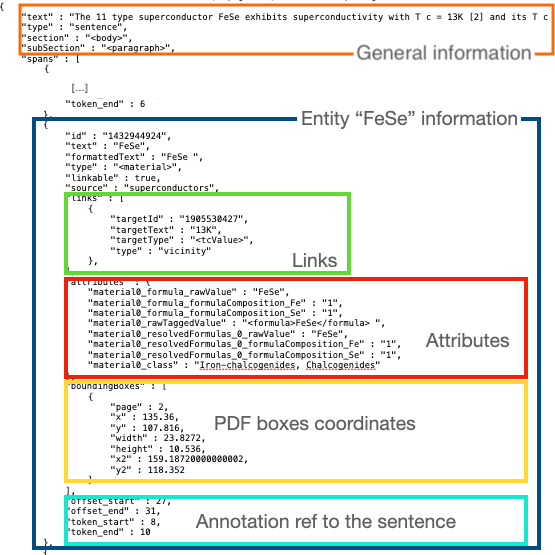
\includegraphics[width=0.8\textwidth]{images/data-flow-2} 
  \caption{Example of the information from one single entity from a passage extracted in the "Extraction Task". The different structured information are highlighted: links, attributes, PDF boxes coordinates (to visualise annotations on the PDF document), and annotations references within the passage (to visualise annotations on text).}
  \label{fig:data-flow-2}
\end{figure}

Each passage is composed of the following attributes: the text of the passage, the type, of passage (whether it's a sentence or paragraph), the main section: header, body, and annex, and the subsections: title, abstract, paragraph, caption.
Furthermore, a passage contains also the list of spans representing the extracted entities and a list of layout token. 
The spans are characterised by text, type, attributes, a unique identifier, and other internal information (e.g. from which ML model the entity was extracted). 
The attributes are stored as a key-value and mainly contain information extracted by the material parser such as, for example the chemical formula, the structured composition, the material class, and so on.
The layout tokens contain low level information coming from the PDF document: font size, font face, superscript, subscript, bold, italic, and the coordinates within the PDF document. The coordinates are couple of x,y numbers that are used to build annotation "boxes" to encapsulate each token independently (Figure~\ref{fig:pdf-view}) 

The "Aggregation Task" is also processed by grobid-superconductors, using a different REST API URL. Here the input is the structured document and the output is a list of rows and columns of summarised records (Figure~\ref{fig:data-flow-3}). 
The aggregation pivots around the relation materials-Tc and attach additional elements to it. Since the Extraction Task tends to match large entities, and they might contains information of multiple materials, for example, multiple records are created. For example, the raw material "Zn and CU doping La Fe B", results in two records (doping: Zn, formula: La Fe B) and (doping:Cu, formula: La Fe B). 
Each record span have its own unique identifier which are calculated using the span attributes such as text, offsets, type, etc. 

\begin{figure}
  \centering
  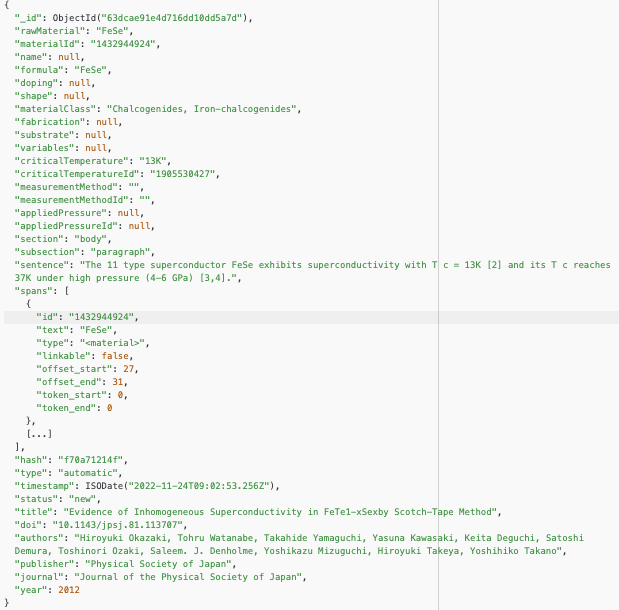
\includegraphics[width=0.8\textwidth]{images/data-flow-3} 
  \caption{Example of record related to the FeSe material after the aggregation.}
  \label{fig:data-flow-3}
\end{figure}

\section{User interface}
\label{sec:user-interface}

The SuperCon\textsuperscript{2} curation interface offers several key features to facilitate the data curation process.
It provides a comprehensive view of materials and their related properties as a table which includes search, filtering, and sorting functionality (Figure~\ref{fig:curation-interface-database}). 
The schema consists of two main classes: material information (material names, formulas, shape, etc.) and properties (T\textsubscript{c}, applied pressure, measurement method, etc.). The complete list including examples is reported in our previous work~\cite{lfoppiano2023automatic}.

\begin{figure}[ht]
  \centering
  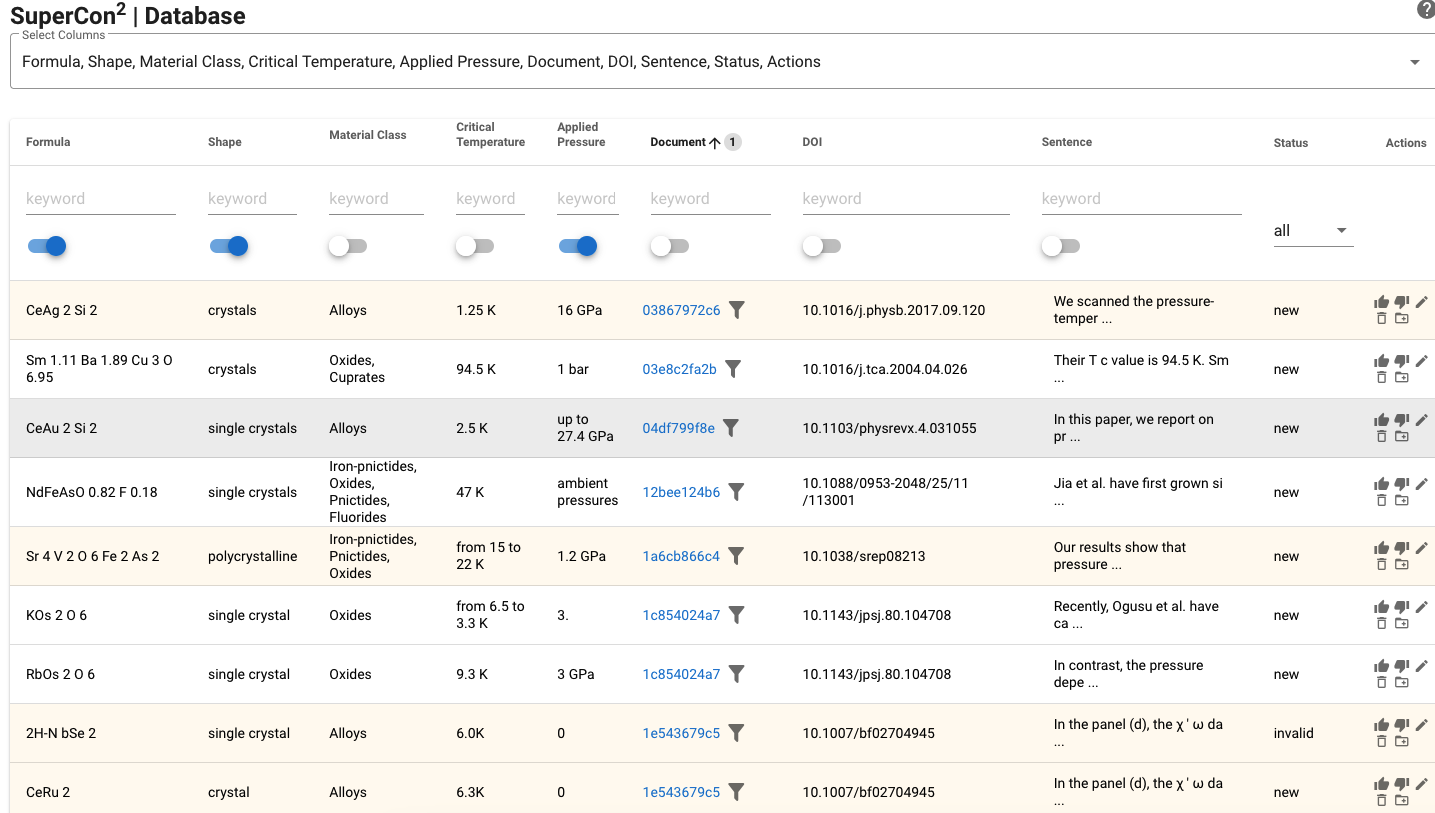
\includegraphics[width=1\textwidth]{images/supercon-curation-database} 
  \caption{Curation interface showing the database as a table}
  \label{fig:curation-interface-database}
\end{figure}


During the curation process is often necessary to navigate back and forth between the the extracted record that is being examined and the related context in the paper (the related paragraph or sentence). 
The curation interface provides a document viewer combining a table with the extracted records and the viewer of their respective document (Figure~\ref{fig:pdf-view}). The viewer highlights the annotations that identify materials and properties, enabling users to easily locate and reference the extracted information within the document.

Users can add, amend, remove, or mark the records that are presented to them.  
Marking a record refers to the act of applying a visual or symbolic indication to a specific record, which can be "invalid" or "validated". 
Adding new records is limited to documents already in the database.

The interface automatically collects training data, when a record is amended, the information pertaining it's raw source information (sentence text, annotations) are collected. 

\begin{figure}[ht]
  \centering
  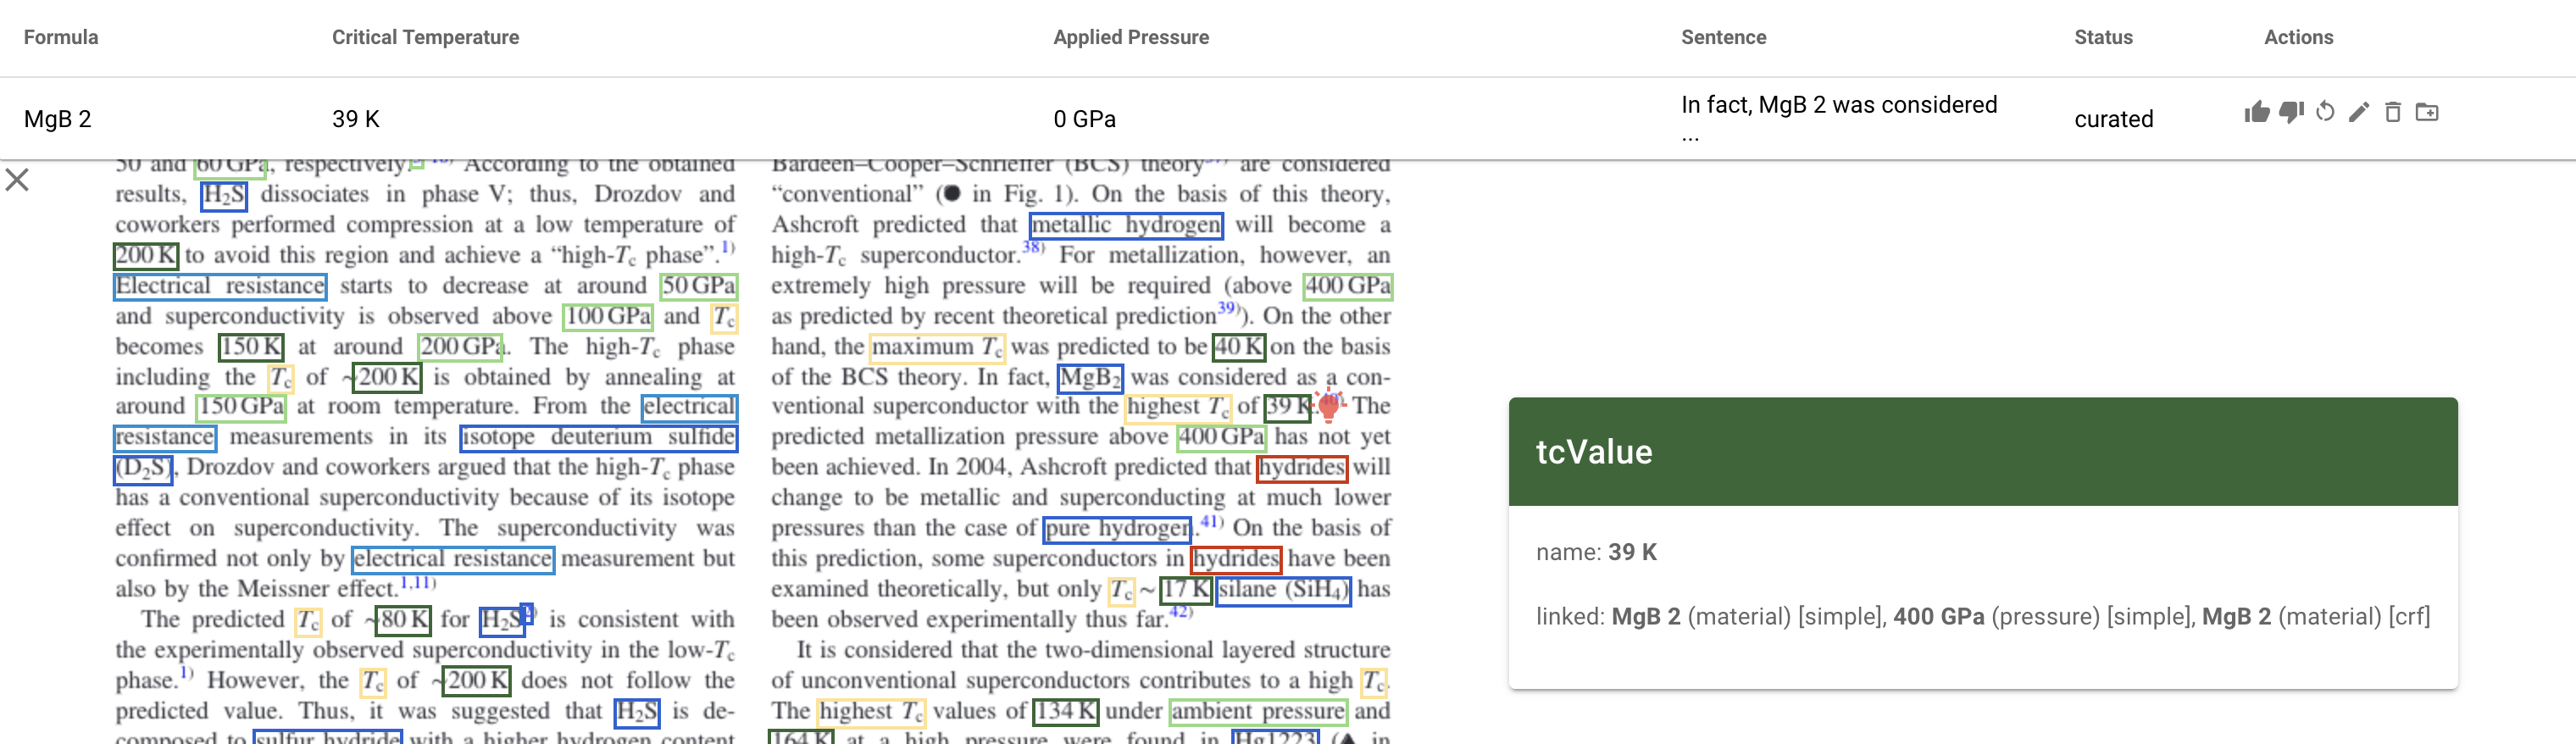
\includegraphics[width=1\textwidth]{images/pdf-view-context.png} 
  \caption{PDF document viewer showing an annotated document. The table on top is linked through the annotated entities. The user can navigate from the record to the exact point in the PDF, with a pointer (the red bulb light) identifying the context of the entities being examined. }
  \label{fig:pdf-view}
\end{figure}

% \begin{figure}[ht]
%   \centering
%   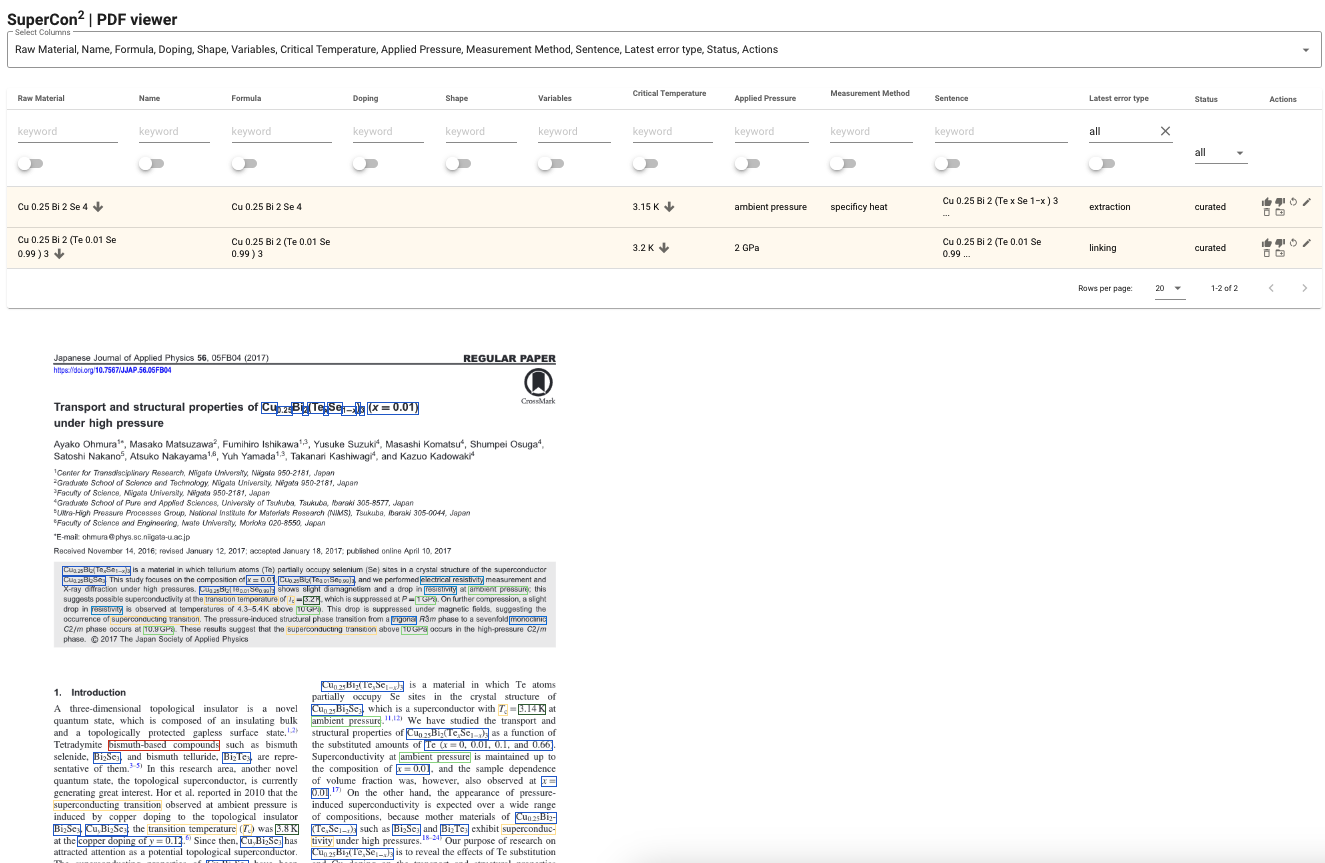
\includegraphics[width=1\textwidth]{images/supercon-curation-pdf-viewer} 
%   \caption{PDF viewer. The page includes a table showcasing records extracted from the  current document, along with the PDF content and accompanying annotations.}
%   \label{fig:curation-interface-pdf-viewer}
% \end{figure}

\subsection{Design principles}
\label{subsec:design-principles}

The design principle is a set of rules we chose at the beginning of the development. We define "curation" the overall process of correcting and validating information, and "correction" the process of modifying the values of a single item. 

\paragraph{Blind curation}
This interface has been built without any multi-user mechanism. 
The data is allocated to different curators by generating randomised links to the application. Each link opens records extracted from a specific document. 
The justification for this approach is twofold: a) the allocation is totally random and each curation does not know any information about the others, and b) the multi-user implementation requires a large effort without any particular scientific gain. 

\paragraph{Data-driven architecture} When a record is amended, the corrected information are stored in a new entry linked to the original one. 
Similarly, when a record is deleted, only its status is modified as "removed", and the record is hidden. 
With this approach we preserve any information, allowing also to generate time series of modified curation records such as which field was corrected, when, and how many changes were done. 
Such information allows the implementation of undo/redo functionality without changes in the data model, if needed in the future. 

On the contrary, original PDF documents, are not duplicated, to save disk space and using the original document hash (Section~\ref{sec:architecture}) as unique identifier.
Obviously, this does not avoid loading two different PDF documents of the same article, because the hash code would be different. In such cases, the anomaly detection (Section~\ref{subsec:anomaly-detection} will detect the duplication by checking the duplication by bibliographic data. 


\begin{figure}[ht]
  \centering
  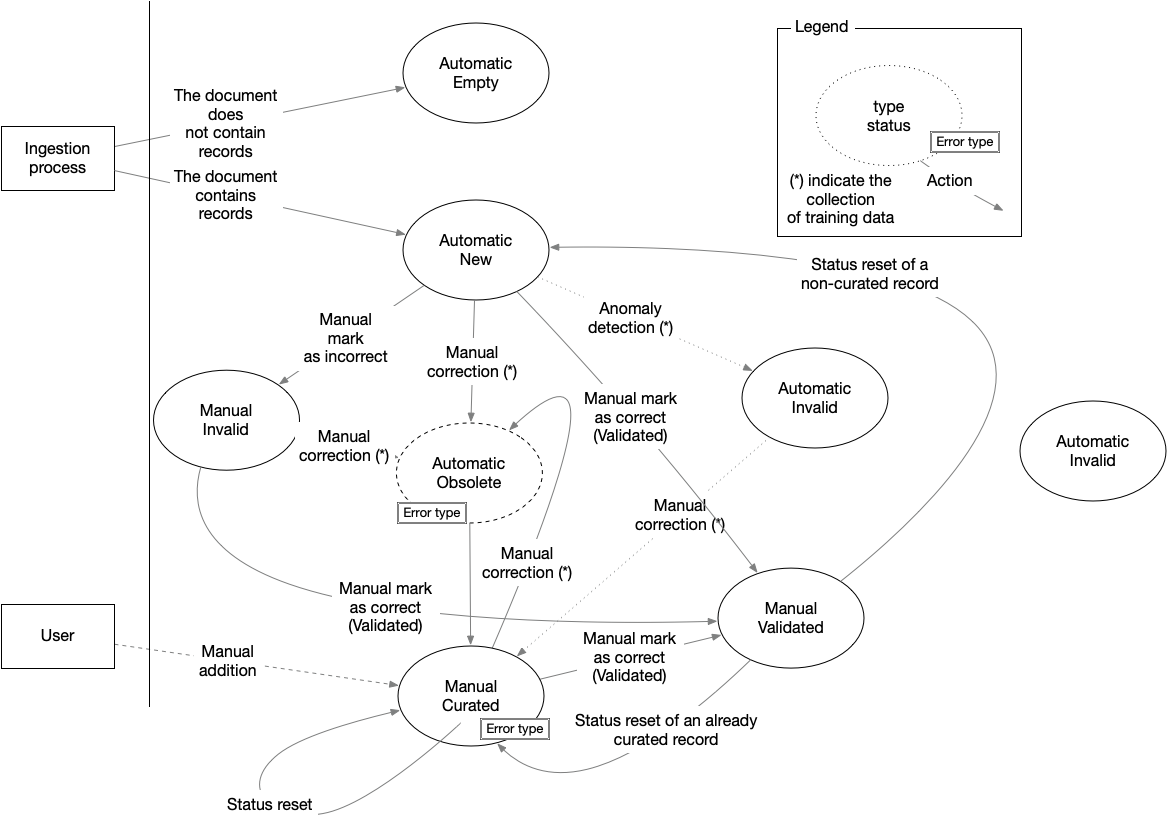
\includegraphics[width=1\textwidth]{images/record-correction} 
  \caption{Schema of the curation workflow. Each state is characterised by two properties: type and status, and one action, as indicated in the top right corner. "Error type" indicates the action of storing the error type for that specific action.}
  \label{fig:curation-workflow}
\end{figure}

\paragraph{Type and Status} Each \textit{record} has two workflow-related fields which are combined to identify the state of the workflow, which is illustrated in Figure~\ref{fig:curation-workflow}. 
The status indicates the record curation status from the data point of view (e.g. validated, invalid, curated, etc.), and is summarised in Table~\ref{tab:record-status}

\begin{table}[htbp]
\centering
\begin{tabular}{|p{2cm}|p{10cm}|}
\hline
\textbf{Status} & \textbf{Description} \\
\hline
new & Default status when a new record is created. \\
\hline
curated & The record has been amended manually. \\
\hline
validated & The record was validated manually. \\
\hline
invalid & The record is wrong or inappropriate for the situation (e.g., T\textsubscript{m} or T\textsubscript{curie} extracted as superconducting critical temperature). \\
\hline
obsolete & Assigned to a record when it is modified, triggering the creation of a new record (internal status, not visible to users).\\
\hline
deleted & The record has been removed by a curator (internal status, not visible to users). \\
\hline
\end{tabular}
\caption{Record status definitions}
\label{tab:record-status}
\end{table}
    
The type indicates whether the record has been created or modified, manually or automatically. 
For example, the value "automatic" is provided when the data is loaded or when the anomaly detection performs some operations. In all other cases it is flipped to "manual". 

\paragraph{Error types} Error types were first introduced in~\cite{lfoppiano2023automatic} while performing manually the end-to-end evaluation. They were combined with the evaluation to provide more detailed information on the reasons why certain extracted values were not correct. 
Since such statistics demonstrated to be useful during the development, we have extended the scope to add additional values related to data curation and validation (Table~\ref{tab:error-types}).

\begin{table}[htbp]
\centering
\begin{tabular}{|p{4cm}|p{8cm}|}
\hline
\textbf{Name} & \textbf{Description} \\
\hline
From table & The entities Material $\rightarrow$ Tc $\rightarrow$ Pressure are identified in a table. At the moment, table extraction is not performed. \\
\hline
Extraction & The material, temperature, and pressure are not extracted (no box) or extracted incorrectly. \\
\hline
Linking & The material is incorrectly linked to the Tc given that the entities are correctly recognized. \\
\hline
Tc classification & The temperature is not correctly classified as "superconductors critical temperature" (e.g., Curie temperature, Magnetic temperature...). \\
\hline
Composition resolution & The exact composition cannot be resolved (e.g., the stoichiometric values cannot be resolved). \\
\hline
Value resolution & The extracted formula contains variables that cannot be resolved, even after having read the paper. This includes when data is from tables. \\
\hline
Anomaly detection & The data is automatically modified by the anomaly detection script. \\
\hline
Curation amends & The curator is updating the data which does not present issues due to the automatic system. \\
\hline
\end{tabular}
\caption{Summary of error type values and description.}
\label{tab:error-types}
\end{table}

In the curation interface, we made the error type mandatory anytime the record is amended or removed. 
Since often the modifications are not related to a mistake, e.g. adding a space in a formula to make it more clear, or replacing garbled characters, we allow an additional error type called "Curation amend" which indicates that the problem is not related to the automatic system. This covers also the case where the modification corrects a mistake from another curator. 
When the update is made, a new record is created, and the error type is stored in the previous record. The workflow schema in Figure~\ref{fig:curation-workflow} indicate "error type" in the states that require its selection. 

\subsection{Usability}
The criteria for evaluating the usability of a user interface can vary depending on the context and specific goals of the evaluation. 
In regard to SuperCon\textsuperscript{2}, the simplicity makes it easier to evaluate, considering the main requirement being a smooth transition between the database records and the context in the document. 
We consider the WEBUSE (WEBsite USability Evaluation Tool)~\cite{chiew2003webuse} evaluation criteria for our analysis. WEBUSE has been considered for evaluating web pages usability in many works and it can be summarised as follows: 
\begin{itemize}
    \item Content, organisation, and readability. The usability of a user interface can be evaluated based on how well the content is presented (clear and concise information) and organised (logical organisation), and how easily readable it is. 
    \item Navigation and links. The ease of navigation and the effectiveness of links within the user interface are important criteria for usability evaluation. 
    \item User interface design. The interface should be visually pleasing and visually consistent throughout the application or website. 
    \item Performance and effectiveness. Performance and efficiency in making the users achieve their goals.
\end{itemize}

We discuss the four criteria as follows. 
\paragraph{Content, organisation and readability} The interface is simple and organised in two main pages: database and document. Since the database contains many columns we have reduced the ones visible by default, to make the table fitting on the average screen. We use colours to separate records belonging to different documents. 

\paragraph{Navigation and links} The interface was designed with a minimalist approach. 
There are links and shortcuts in many duplicated positions to reduce the effort for certain repeated actions.
Finally, we provide an alternative and more efficient approach to navigation and correction using only the keyboard. 

\paragraph{User interface design}
The user interface is designed on top of the Vue.js JavaScript framework~\footnote{footnote needed}.  
Vue.js enables reactive operations such as text input and filtering. 
Additionally, it adopts the Vuetify design framework\footnote{footnote needed}, which adheres to Google's recommended Material Design principles.
These principles promote a unified and responsive user interface that incorporates elements inspired by physical materials ultimately aiming to create a delightful and engaging user experience.

\paragraph{Performance and effectiveness}
We designed the interface to reduce the actions required by users to transition from the record to the contextual information. 
The context is accessible in two ways: in the database view (Figure~\ref{fig:curation-interface-database}) we provide as column in each record, the sentence in which the record belong, decorated with colours for each annotation relevant to the record.
In the document view, the users can quickly move from the table to the related part of the PDF document, enhanced with the extracted annotations (Figure~\ref{fig:pdf-view}). 
These solutions should reduce the time used to search information in the document. 

\subsection{Curation and processing logs}
\label{subsec:curation-and-processing-logs}

The Supercon\textsuperscript{2} interface give access to information regarding the ingestion (processing log) and the curation process (curation log). 
The processing log is filled-up when the data is ingested, it was build to have minimal functions able to explain why certain documents haven't been processed (Figure~\ref{fig:processing-curation-log}). 
For example, sometimes documents are failing because they don't contain any text (image PDF documents) or they are too big (more than 100 pages). 
% Grobid was built focusing on speed and robustness, and contains several fail-safe mechanisms to avoid crashing the system when a document is either too big or does not contains valuable information, for example does not have any text. 
% Old PDF documents (e.g. before 1990) are likely have been scanned and contains only images. 
% Examples of too big documents are dissertation thesis with more than 100 pages, that might be collected by mistake. 


\begin{figure}[ht]
  \centering
  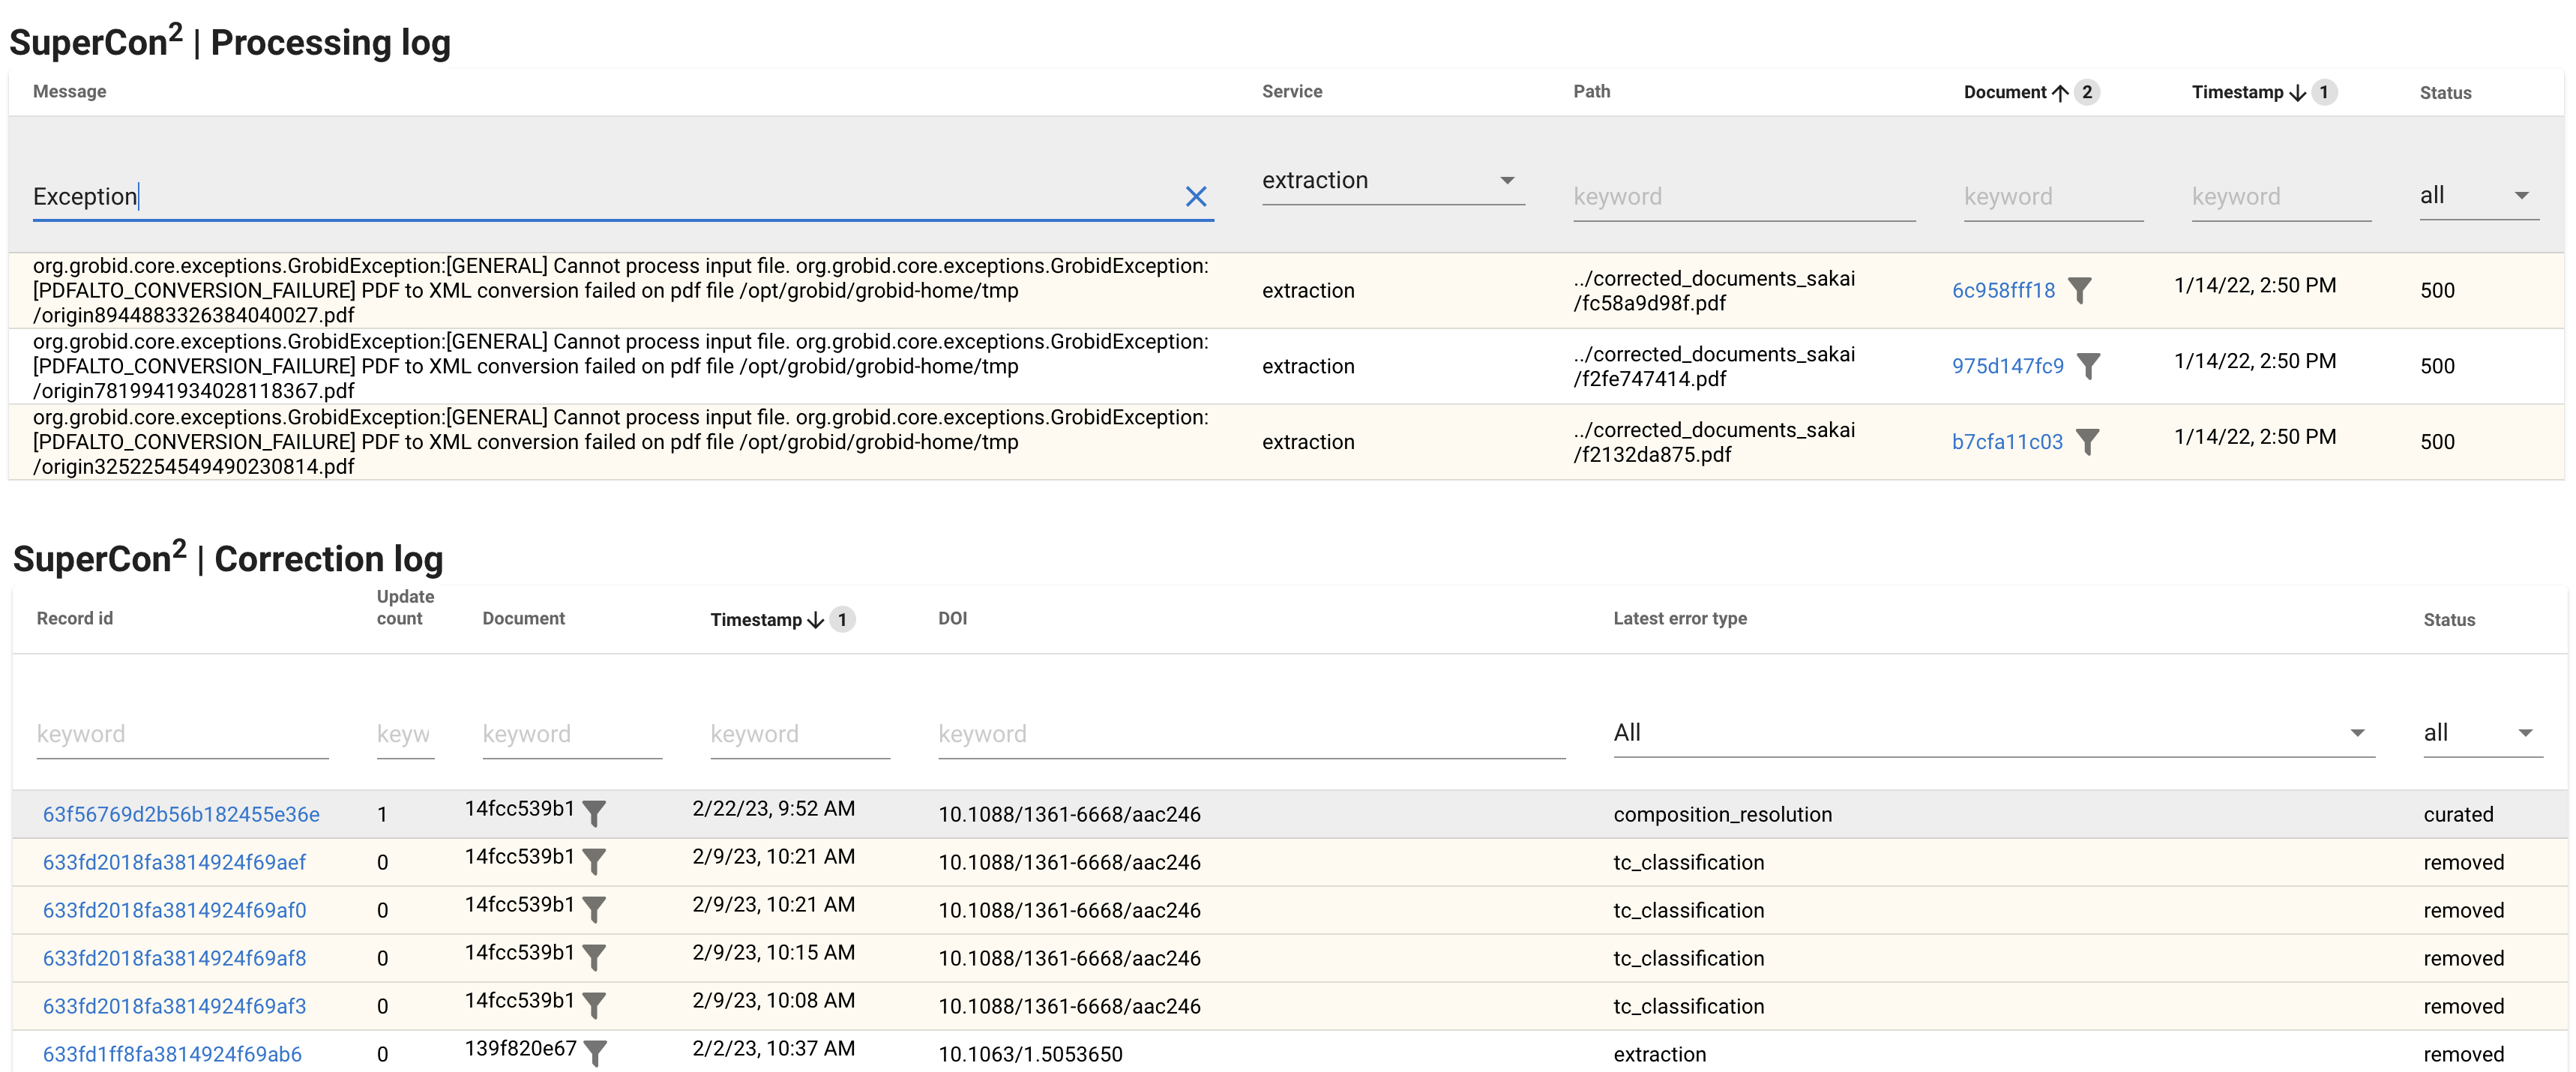
\includegraphics[width=1\textwidth]{images/processing-curation-log.png} 
  \caption{On the top: Processing log, showing the output of each operation (process document, create a record) and the outcome with the exception or error that should have occurred. On the bottom: Curation log, indicating each record, the number of updates, and the date/time of the last updates.}
  \label{fig:processing-curation-log}
\end{figure}

The curation log provides a view of what, when and how a record has been corrected (Figure~\ref{fig:processing-curation-log}).

% \begin{figure}[ht]
%   \centering
%   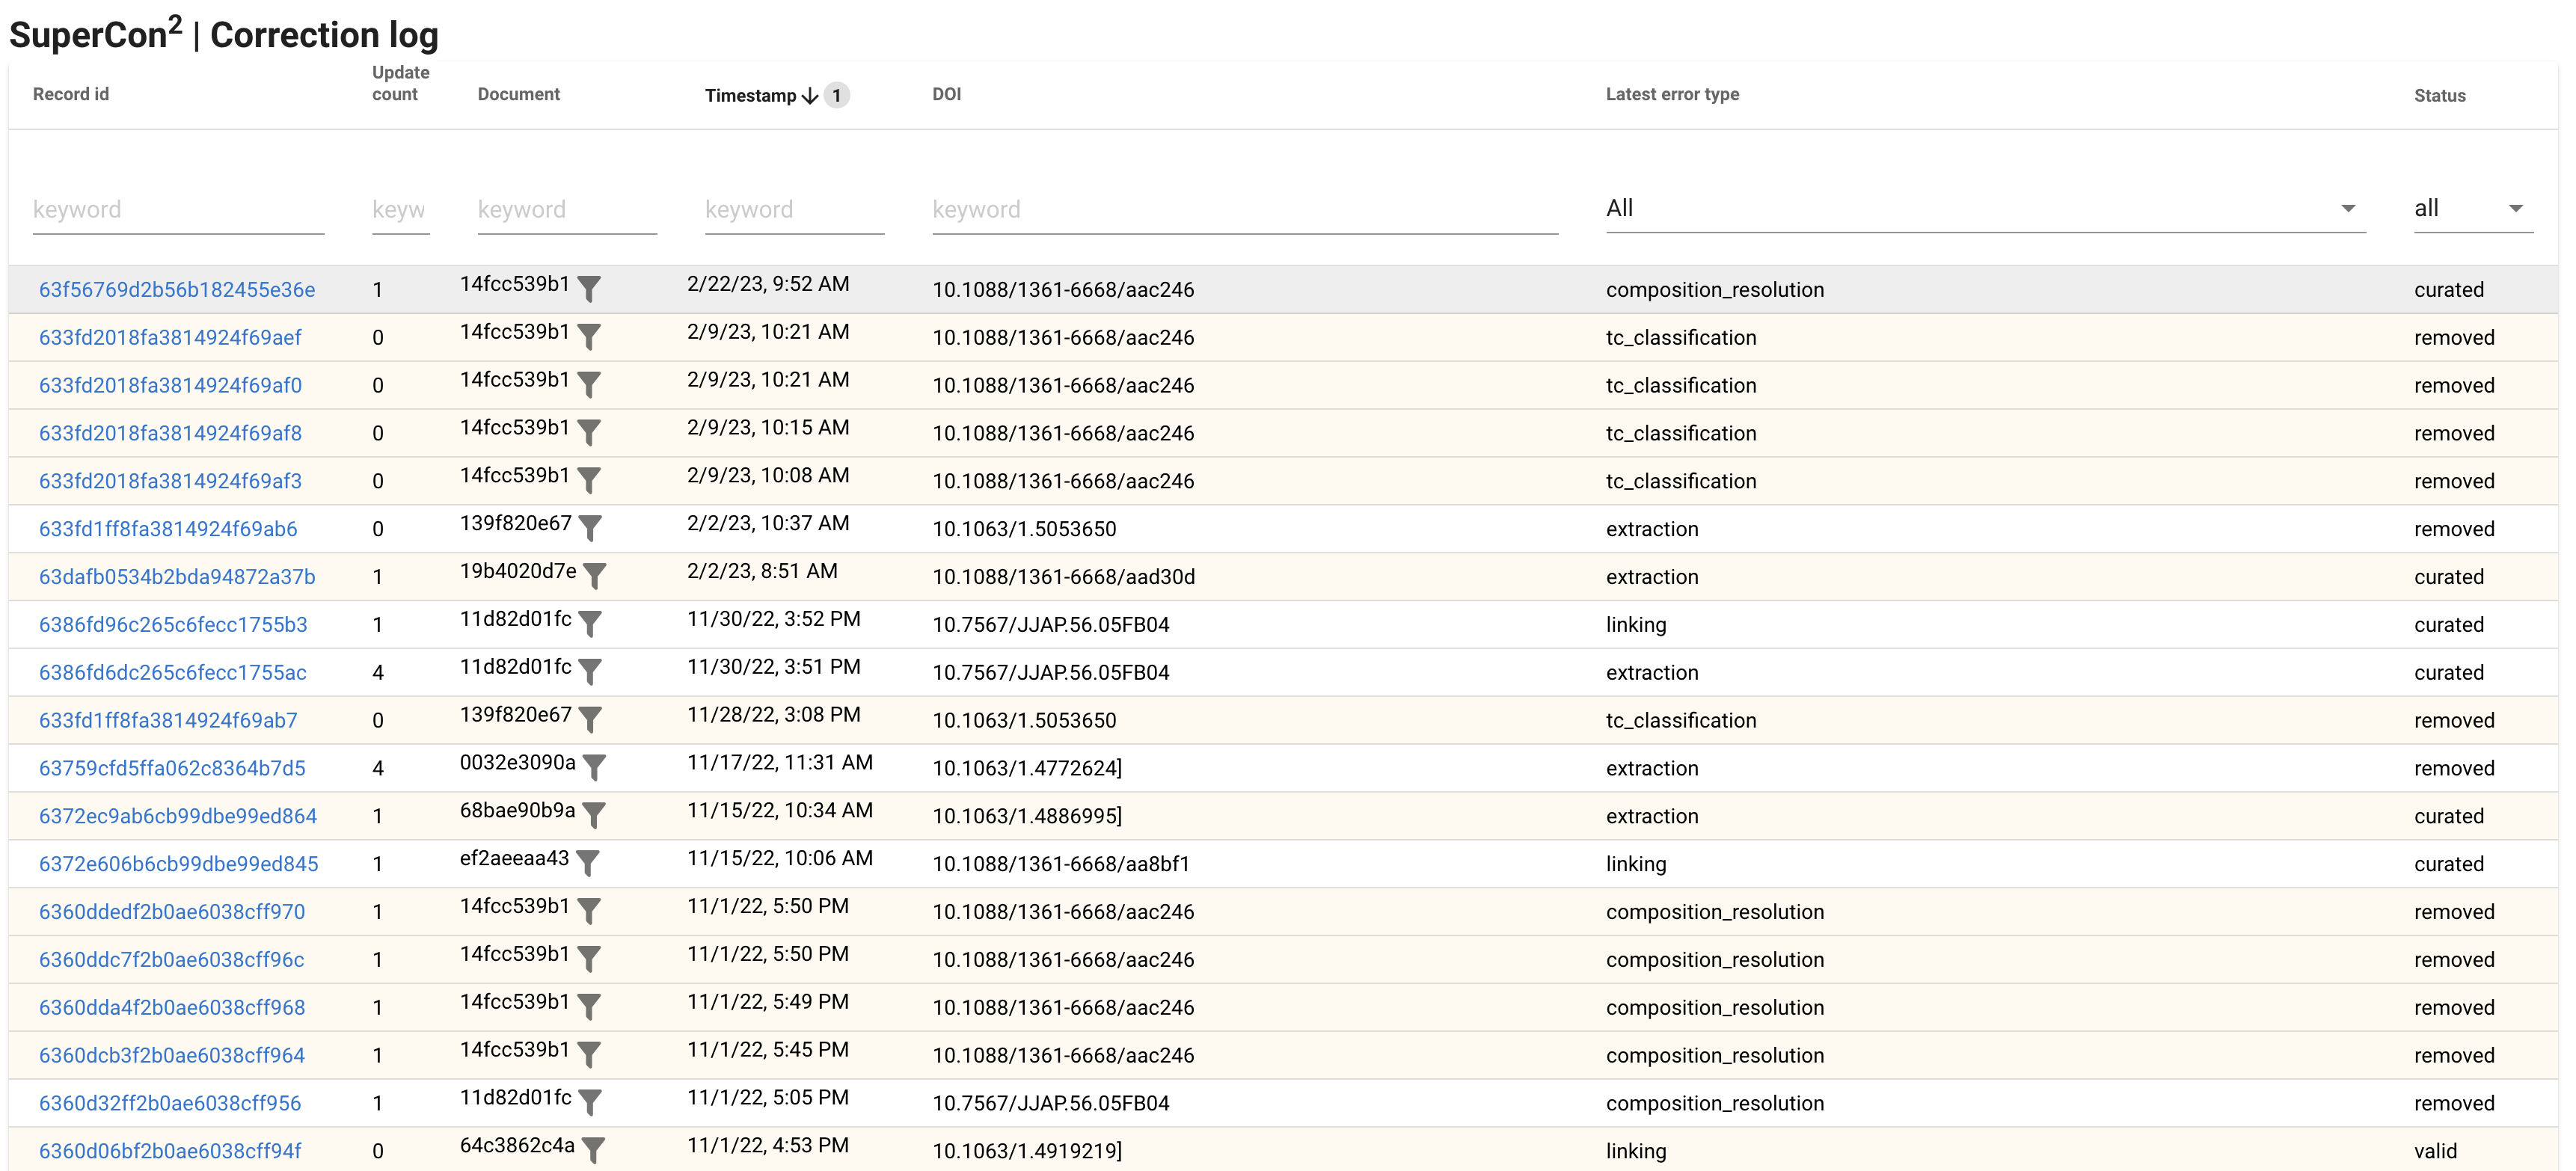
\includegraphics[width=1\textwidth]{images/curation-log} 
%   \caption{Curation log, indicating each record, the number of updates, and the date/time of the last updates. }
%   \label{fig:curation-log}
% \end{figure}


\section{Data correction for automatically extracted entities in SuperCon\textsuperscript{2}}
\label{sec:data-correction}

In this section, we describe the processes related to data correction using the user interface. 
First, (Section~\ref{subsec:anomaly-detection}) we discuss anomaly detection as the pre-processing phase. 
Then, the manual correction process is described in Section~\ref{subsec:manual_correction}. 
At each correction, we collect data to be fed back as training data to the ML model, which is covered in Section~\ref{subsec:feedback-loop-training-data}.

\subsection{Anomaly detection}
\label{subsec:anomaly-detection}
Anomaly detection is the process of identifying unusual or unexpected events or patterns in data. In this project, we limited the implementation to a few simple rule-based filters focusing on formulas and T\textsubscript{c} values.
We adopted the convention to set the corresponding record status as "invalid" and its type as "automatic" which can be identified by curators when the filter identifies an anomaly. 
The rule marks as "invalid" all the records for which the extracted T\textsubscript{c} is greater than room temperature (273 K) and when the chemical formula cannot be parsed with a standard library. However, stochiometric formulas with variables are still valid, even if they cannot be parsed properly.
It is crucial to stress that these rules should not be too strict  and further validation by curators is necessary. 
We are aware that Tc values above room temperature could be perfectly legit in researchers' hypotheses or preliminary calculations. 
% There are other cases where the anomaly detection could bring more harm than benefits. 
% For example, anomaly detection perpendicularly on the database, aggregating each formula to verify the variation of the related Tc. 
% In SuperCon\textsubscript{2} , when we tried to discover the outliers, we realised that might be a double edge sword.
% The variation can be compared with a certain tolerance, but what is a good value? 
% Whether it's few or several Kelvin, it's hard to establish. 
% If we consider the possibility to extract relative Tc (order of 1-2 K) mixed with absolute Tc (order 0-100 K), the relative Tc will risk to wrongly identify correct values as anomalies.

When the filter was applied to the SuperCon\textsuperscript{2} database, it found 70 records with invalid T\textsubscript{c} and 7000 records that contain invalid formulas whose the majority were due to stochiometric variables. We also identified only 1157 materials with multiple Tc values; after evaluating the possibility to recognise Tc values outliers, within a large tolerance we did not come to any conclusive outcome. 
There are two problems here: first, is the difficulty to a reasonable value to compare multiple Tc values, and the second is found which tolerance is good enough, which is very likely variable depending on the material. 


% For example, if we consider a popular superconductor: Mg B2, which has absolute Tc = 39K and relative Tc around 2-3 K (37-40 K). 
% If we consider 50\% tolerance over the average, if we consider 3 Tc values (39,39,2) on which one is is likely that all the correct values (37-40K) will be out of scale if we try to identify outliers based on the average +- 50\%. 

When processing data from different collections is possible that the same document is wrongly loaded because the PDF is slightly different (e.g. published document and pre-print document) under different MD5 hashes.  
We apply this filter using the bibliographic data (first by DOI, then by title and authors, etc). This works because the bibliographic data are consolidated before loading a document, therefore a pre-print and a published document will obtain the exact same bibliographic data.


\subsection{Manual correction}
\label{subsec:manual_correction}
The manual correction is still indispensable for developing high-quality structured data, since the automatic extracted data is not perfect as discussed in \cite{lfoppiano2023automatic}, and the anomaly detection (Section~\ref{subsec:anomaly-detection}) only detects potential problems. 
We employ only domain-experts as curators in order to certify the correctness of the data outcome. 
To avoid worker dependence and ensure robustness in the process, we took two approaches. 
First, we used a double-round approach where the data is initially corrected by one person, and validated in a second round, by a different person. 
Second, we have built documentation for the curation as form of guidelines through an iterative loop of processes, as discussed in our previous work on the construction of the annotated dataset SuperMat~\cite{foppiano2021supermat}. 
The loop includes four steps: (i) collect rules, based on observation and reasoning, (ii) curation following those rules (iii), retrospective including analysis and discussions based on curators feedback, and (iv) take decisions and update the guideline.

The guidelines consist mainly of two parts: the general principles and the correction rules with examples of solutions.
The guidelines are designed to provide general information applied to corrections and very basic explanation containing illustrations for a faster understanding (e.g. the meaning of the colours of the annotations). This would help new curators to catch up with the required level of curation precision quickly. 
There are two main components described in the correction rules: the record that is being corrected and its context. 
The context of a record can be obtained by examining the extracted annotated text or the PDF document area.

The correction rules are described based on the error type mentioned in Section~\ref{subsec:design-principles}, and in the guideline the description of rules are accompanied by sheets that explain five points to the curators, as illustrated in Figure~\ref{fig:example-curation-sheet}:
\begin{itemize}
    \item \textbf{Sample input data}, a screenshot of SuperCon\textsuperscript{2} record in the interface
    \item \textbf{Context}, a screenshot of the related part of the document (either from the PDF or from plain text sentences) that contain the extracted data to be curated,
    \item \textbf{Motivation}, describes the issue with the extracted data in exam, 
    \item \textbf{Action} to be taken, 
    \item \textbf{Expected output}, a screenshot of the expected SuperCon\textsuperscript{2} record, after correction
\end{itemize}

% An example of a sheet can be found in Figure~\ref{fig:example-curation-sheet}. 

\begin{figure}[ht]
  \centering
  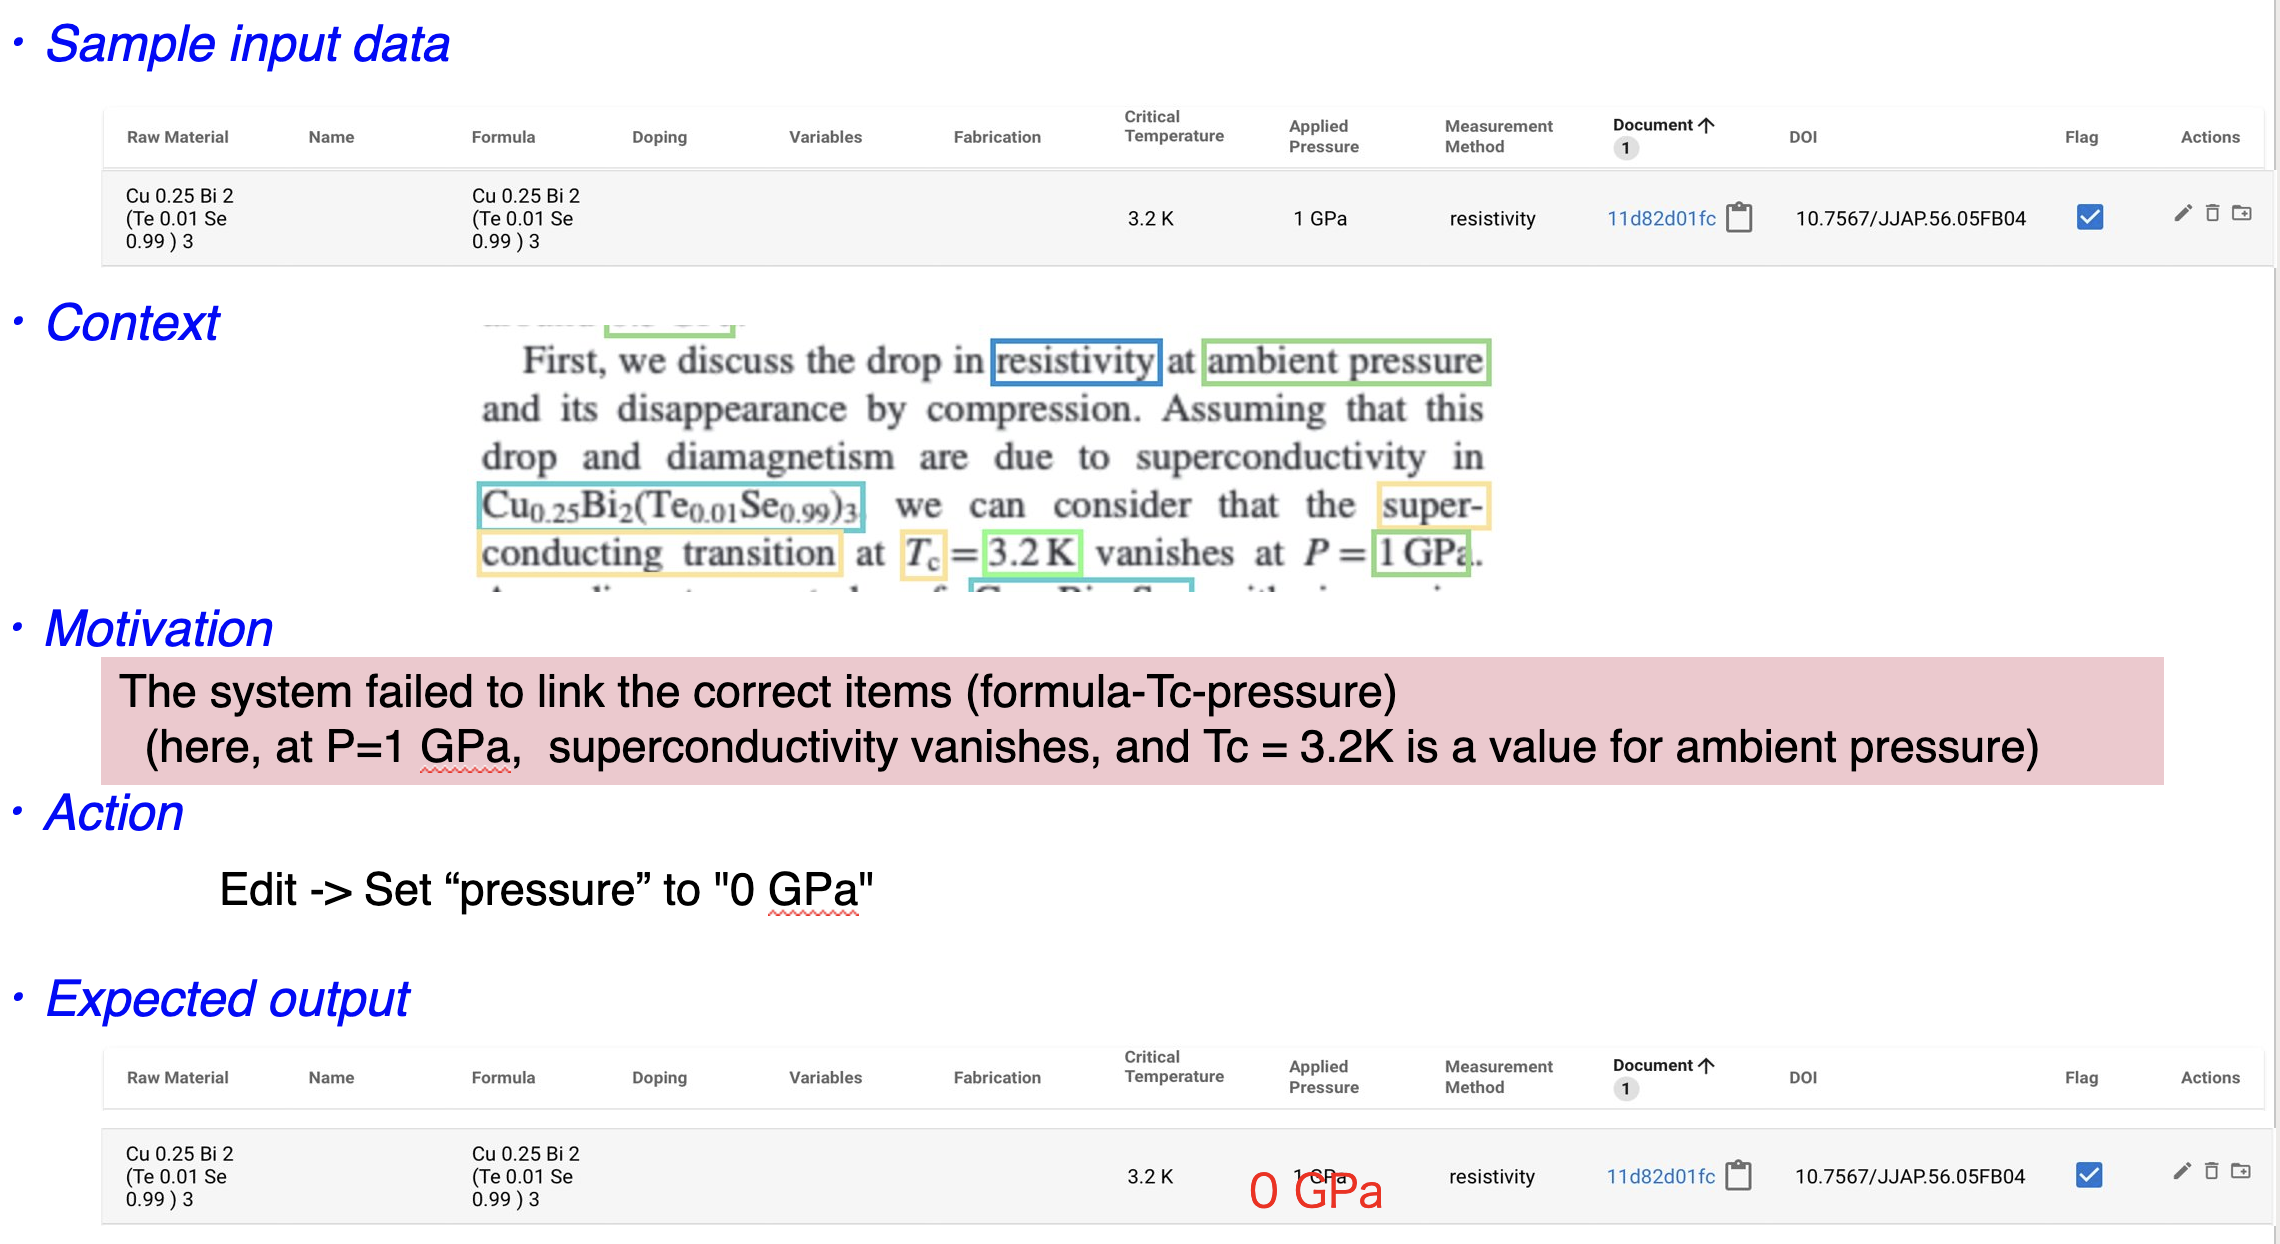
\includegraphics[width=1\textwidth]{images/example-sheet-curation.png} 
  \caption{Example of curation sheet. As discussed, it's written with simple language assuming the curator may not be familiar with the task. }
  \label{fig:example-curation-sheet}
\end{figure}


\subsection{Automatic training data generation}
\label{subsec:feedback-loop-training-data}
The curation process is a valuable endeavour that requires significant knowledge and human effort. It is crucial to maximize the utilisation of this time to extract as much information as possible. 
For this reason, we integrated the automatic collection of source data in the curation process. This allows to retrieve training data related to mistakes corrected by curators and  feed back as training data to the ML model. 

When a correction is performed:
\begin{itemize}
    \item the new record with updated information is prepared and stored, 
    \item if the data for this passage has already been created (e.g. another correction within the same sentence was already performed), then the data is not collected,
    \item using the record document identifier (the hash), the latest structured document is retrieved from the document collection,
    \item using the record "materialId" the exact span (representing the single annotated entity) is searched within the structured document,
    \item when the material is found, then the whole passage object containing the text string, spans, tokens and other information are collected and saved in a separate collection. The curated record id is also attached to the training data 
    \item the data can be used to generate a text with the annotated entities using the spans list and the feature files using the tokens list.
\end{itemize}

The training data can be inspected in a specific page of the application (Figure~\ref{fig:training-data-view}) and sent to the training data annotation tool. We integrated our interface with label-studio~\cite{Label_Studio} which is an open-source and flexible interface. 
Examples are visualised by rows with their document hash and the status which can be "new" when the data is just added or "in progress" after the data is sent to the label-studio application. 
The workflow does not require additional states, because the data can be exported from label-studio after corrected. 

\begin{figure}[ht]
  \centering
  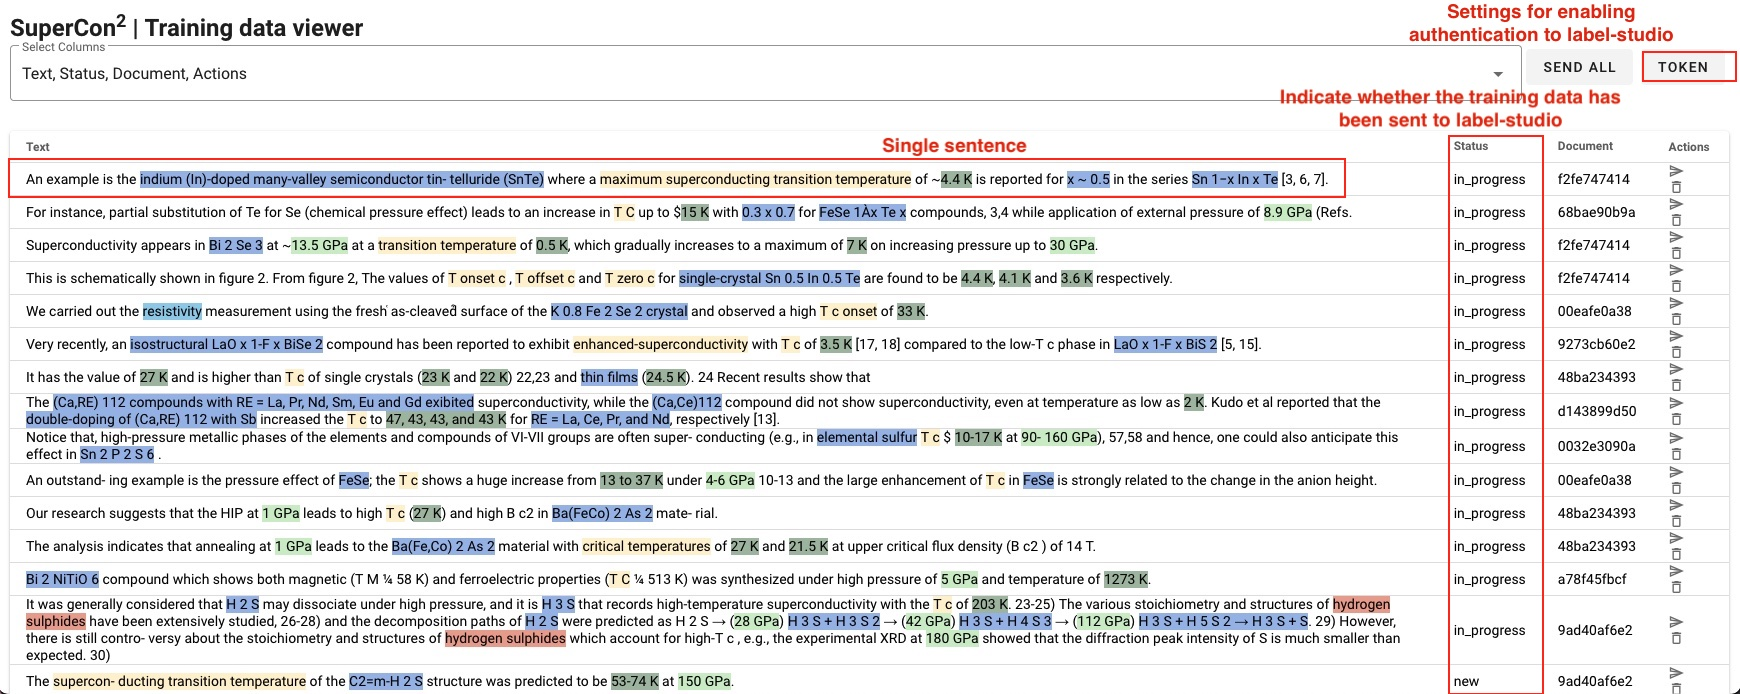
\includegraphics[width=1\textwidth]{images/training-data-viewer} 
  \caption{Training data view}
  \label{fig:training-data-view}
\end{figure}

Since the training data generated with this interface are related to manually corrected mistakes in the TDM process, intuitively, they should provide a higher impact in improving the model than training data of the same amount, randomly selected.
To prove this hypothesis, we performed an experiment: we selected around 400 records initially marked as incorrect by the anomaly detection script and we curated them. 
Then, we curate the related training data we obtained a set of 352 examples (we excluded the examples for which no correction was performed). 
We define as \textit{curation} the dataset from curated data and as \textit{base} the original SuperMat dataset.

In this experiment we focused on the best model, which is based on SciBERT~\cite{Beltagy2019SciBERT}. 
We use the DeLFT (Deep Learning For Text)~\cite{DeLFT} library for training, evaluating, and using the models for prediction. 
We can train a model using two different strategies: "from scratch" when the model is initialised randomly (s) or "incremental" when the initial model weights are taken from an already existing model (i).
The latter can be seen as a way to "continue" the training from a specific checkpoint. 
We defined three scenario: a) base from scratch, b) base+curation from scratch, and c) base+curation incrementally. 
We merge curation with the base dataset because the curation dataset is very small as compared with base, to avoid forgetting previous weights.  

The obtained models are tested using a fixed holdout dataset we have designed in our previous work~\cite{lfoppiano2023automatic} and the evaluation scores are illustrated in Table~\ref{tab:evaluation-curation-training}.

\begin{table}[ht]
\centering
\begin{tabular}{|l|l|l|l|}
\hline
& \textbf{Base} & \textbf{base+curation(s)} & \textbf{base(s)+curation(i)} \\ 
\hline
\hline
Nb total examples & 16902 & 17254 & 16902(s), 17254 (i)\\ 
\hline
\texttt{<class>}        & 70,22             & 72,30             & \textbf{72,63} \\ 
\texttt{<material>}     & 79,69             & 80,23             & \textbf{80,61} \\ 
\texttt{<me\_method>}   & 64,78             & 65,31             & \textbf{66,62} \\ 
\texttt{<pressure>}     & \textbf{46,96}    & 46,53             & 46,84 \\ 
\texttt{<tc>}           & 77,36             & 78,56             & \textbf{79,57} \\ 
\texttt{<tcValue>}      & 77,26             & \textbf{77,94}    & 77,84 \\ 
\hline
\textbf{All (micro avg.)} & 75,86           & 76,66             & \textbf{77,36} \\ 
\hline
\textbf{Diff avg. w/ baseline}& -           & +0,80             & \textbf{+1,50} \\ 
\hline
\end{tabular}
\caption{F1-score from the evaluation of the fine-tuning training of SciBERT. 
The training is performed with three different approaches. 
The Base dataset is the original dataset described in~\cite{lfoppiano2023automatic}, the curation dataset is automatically collected based on the database corrections by the interface and manually corrected. \textit{s} indicate "training from scratch", while \textit{i} indicate "incremental training". 
The evaluation is performed using the same holdout dataset from SuperMat. 
The results are the average of 5 repeated train-evaluation runs. }
\label{tab:evaluation-curation-training}
\end{table}

The result of this experiment is that with only 352 examples (0.002\% of the SuperMat dataset) we obtained an improvement of +1.50\% F1 score. The incremental approach obtained almost twice the improvement of the model trained from scratch with the extended dataset. 
There are several hypotheses for this, one could argue that the dataset is not big enough for the task at hand, therefore the model requires more training time. This issue could be verified by correcting all the available training data and repeating this experiment. 

\section{Interface evaluation}
We conducted an experiment to compare the efficiency and correctness of data extraction using two methods: a) the SuperCon\textsuperscript{2} user interface or b) the "traditional approach" of reading PDF documents and filling up an Excel file. 
Our sample consisted of 15 papers, which were distributed among three curators — a senior researcher, a PhD student, and a master student. 
Each curator received 10 papers, with an equal split between the two methods. Each paper was shared among two curators, each of them with different method: interface vs PDF document. 

We evaluated the two methods based on two trade-off aspects: efficiency, by comparing the time required for curation, and accuracy, measured in terms of precision, recall, and F1-score.

The comparison of the time taken revealed no significant difference between the interface and the traditional method. Specifically, the total time was only 4 minutes longer with the interface (188 minutes compared to 184 minutes). The time difference did not demonstrate any consistent trend, suggesting the need for a larger dataset in future experiments.

When we examined the accuracy of the extracted data, we observed a 5\% improvement in precision and a substantial 50\% improvement in recall when using the interface (Table~\ref{tab:evaluation-interface-correction}). 

\begin{table}[ht]
\centering
\begin{tabular}{c|ccc}
    & \textbf{P (\%)} & \textbf{R (\%)} & \textbf{F1 (\%)} \\
    \hline
    PDF document & 87.83 & 45.60 & 52.66 \\
    Interface & \textbf{93.37} & \textbf{96.39} & \textbf{93.28} \\
\end{tabular}
\caption{Results of the comparison between the curation using the SuperCon 2 interface and the traditional method of reading the PDF document. }
\label{tab:evaluation-interface-correction}
\end{table}

The disparity in experience significantly influenced the accuracy of curation, particularly in terms of high-level skills. Senior researchers consistently achieved an average F1-Score approximately 15\% higher than other curators (see Table~\ref{tab:accuracy-by-experience}). 
Furthermore, we observed a modest improvement between master students and PhD students. These findings indicate that employing master students could be a cost-effective alternative to PhD students, with comparable outcomes.

\begin{table}[h]
\centering
\begin{tabular}{c|ccc}
\textbf{Experience} & \textbf{P (\%)} & \textbf{R (\%)} & \textbf{F1 (\%)} \\
\hline
Master student & 90.03 & 66.10 & 66.40 \\
PhD student & 83.33 & 65.69 & 69.45 \\
Senior researcher & \textbf{98.45} & \textbf{81.22} & \textbf{83.08} \\
\end{tabular}
\caption{Accuracy measured by curator experience}
\label{tab:accuracy-by-experience}
\end{table}

Finally, the collected data suggests that all three curators had overall more corrected results by using the interface as illustrated in Table~\ref{tab:accuracy-by-experience-method}. 

\begin{table}[h]
\centering
\begin{tabular}{c|cccc}
\textbf{Experience} & \textbf{Method} & \textbf{P (\%)} & \textbf{R (\%)} & 
\textbf{F1 (\%)} \\
\hline
\multirow{2}{*}{Master student} & PDF Document & 94.58 & 36.55 & 48.67 \\
 & Interface & 83.19 & 95.83 & 88.25 \\
\hline
\multirow{2}{*}{PhD student} & PDF Document & 70.00 & 48.51 & 50.78 \\
 & Interface & 96.67 & 82.86 & 88.11 \\
\hline
\multirow{2}{*}{Senior researcher} & PDF Document & \textbf{100.00} & 55.56 & 61.03 \\
 & Interface & 97.42 & \textbf{98.33} & \textbf{97.78} \\
\end{tabular}
\caption{Accuracy measured by experience and method, PDF document vs Interface}
\label{tab:accuracy-by-experience-method}
\end{table}


The results of this experiment confirmed that utilizing the interface in conjunction with an automated system required a comparable amount of time for curating SuperCon data compared to the "traditional method." However, it significantly improved the accuracy of the extracted data.
Additionally, several observations were made during the curation process:

\begin{itemize}
    \item The initial work on the first documents took longer when using the interface, primarily due to participants' lack of familiarity with it. Conversely, starting with the PDF document was more straightforward and necessitated less transfer learning.
    \item The interface demonstrated a substantial increase in recall, while there was a tendency to overlook information when reading the PDF document.
    \item Data extracted from the PDF documents exhibited fewer or no instances of duplication, which contrasted with the automatic data.    
\end{itemize}


\section{Code availability}
This application is freely available at \url{https://github.com/lfoppiano/supercon2}, the repository contains:
\begin{itemize}
\item the code of the SuperCon 2 curation interface for visualising and editing material and properties extracted from superconductors-related papers.
\item The ingestion workflow to create process PDF documents with Grobid-superconductors and produce a database of materials and properties.
\item the guidelines, accessible at \url{https://supercon2.readthedocs.io}
\end{itemize}

\section{Acknowledgements}
Our warmest thanks to Patrice Lopez, the author of Grobid~\cite{GROBID}, DeLFT~\cite{DeLFT}, and other open-source projects for his continuous support and inspiration with ideas, suggestions, and fruitful discussions.
We thank Pedro Baptista de Castro for his support during this work. 

\section{Conclusions}
We built a staging area for SuperCon that allow the feeding with high quality data from TDM of materials and properties through an efficient manual curation. 
The data is loaded through an ingestion process that load a persistent database with automatically extracted information of materials and properties through Grobid-superconductors~\cite{lfoppiano2023automatic}. 
The ingestion process employ simple also simple anomaly detection rules to identify outliers.
We then developed a user interface for curate the new superconductors data extracted automatically, before it is sent to the SuperCon database. 
The interface combines the best practices in user interaction design and provides among many features: an enhanced PDF document visualisation, and rapid transitions from the database records the related section in the original document. 
We reported that our interface achieve higher precision while requiring the same time for curating, as compared with the traditional manual process.
The interface also automatically collects data related to correction that can be used to feed back the ML models as training data. 
We demonstrated that the feedback loop based on corrected data can improve substantially the machine learning models with fresh and targeted training data. 

There are several planned features and improvements in the pipeline. Some of these include:

\begin{itemize}
    \item Undo/redo functionality: The ability to undo and redo changes made to records will be added, to make it easier to correct mistakes.
    \item Document versioning: A versioning system will be implemented to track changes to documents over time.
    \item Improved search: The search functionality will be improved to make it easier to find records based on specific criteria.
    \item Additional record types: SuperCon\textsuperscript{2} currently supports records for material and property information, but additional record types will be added in the future.
\end{itemize}

\section*{Contributions}
LF wrote the paper and everybody else revised it. 
LF and POS discussed the ML results and experiments. 
LF wrote the back end, and TM wrote the front end of the user interface. 
LF designed the user interface experiment with KT, TT and WS as curators.
KT lead the materials-science work on the data with CS, TT and WS.
TA revised the paper from CS's perspective.
YT and MI supervised the work. 


\bibliography{references}
\bibliographystyle{unsrt}

\end{document}



